\subsection{Path Planning and Execution}
\label{sec:path-planning}

The navigation stack utilizes a hierarchical approach to move the ASV between waypoints while ensuring obstacle avoidance.

\subsubsection{Hybrid Planning Strategy}
As detailed in the technical report, the \texttt{Planning Node} does not run A* constantly to save on computational overhead. Instead, it follows a multi-stage logic:
\begin{enumerate}
    \item \textbf{Direct Vectoring:} A straight line is projected between the current pose and the target.
    \item \textbf{Proximity Detection:} If an obstacle is detected within \textbf{1.0 m} of this direct path, the system triggers the \textbf{A* algorithm}.
    \item \textbf{Grid Constraints:} The occupancy grid uses a cell size of 0.5 m. Waypoints generated by the planner are enforced to be at least \textbf{2.0 m} (two boat lengths) apart to ensure smooth transitions and prevent erratic steering.
\end{enumerate}

\subsubsection{Control and Following Logic}
The \texttt{Control Node} processes the path into motor commands using heading-based thresholds:

\begin{itemize}
    \item \textbf{Coarse Alignment:} If the heading error exceeds \textbf{45$^{\circ}$}, the vehicle stops forward movement and performs a turn-in-place.
    \item \textbf{Fine Navigation:} Within the 45$^{\circ}$ window, the vehicle moves forward using differential thrust.
    \item \textbf{Differential PID:} The system sets the outside propeller to maximum PWM and modulates the inside propeller speed proportionally to the heading error via a PID controller.
    \item \textbf{Dynamic Rudder Engagement:} Physical rudders are engaged at their optimal \textbf{35$^{\circ}$} angle only when the heading error is sufficiently large, reducing the complexity of the propulsion state space.
\end{itemize}

\begin{figure}[H]
    \centering
    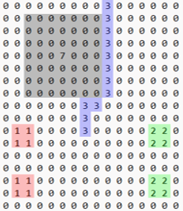
\includegraphics[width=0.6\textwidth]{images/Local_Map_with_Obstacles.png}
    \caption{Local occupancy grid visualization with obstacles (Ref: Technical Report Fig. 9)}
    \label{fig:local-map}
\end{figure}